\chapter{Versuchsdurchführung}

In diesem Kapitel wird der Hardware- und der Softwareafaufbau des Versuches beschrieben.

\section{Versuchsaufbau}

Der Student erhällt folgende Komponenten:
\begin{itemize}
    \item RespberryPi 3
    \item CC2531 Sniffer Stick
    \item cod.m ZigBee CC2652P2 Raspberry Pi Module
    \item 2 x Phillips Hue White E27
    \item 1 x Phillips Hue dimmer switch
    \item HDMI Kabel
    \item Ethernet Kabel
\end{itemize}

Der Student muss KVM Komponenen selbst bereitstellten. Alternativ, wenn der Versuch in der Hochschule durchgeführt werden sollte,
können diese auch durch die Hochschule gestellt werden. Der ZigBee Kordinator ist als \grqq Hat \grqq{} auf dem Raspberry installiert. Der Sniffer ist per USB an der 
Frontseite des Raspberrys angeracht.

\section{Versuchssoftware}

Folgende Software wird eingesetzt:
\begin{itemize}
    \item RaspbianOS
    \item Docker
    \item zigbee2mqtt
    \item mosquitto
\end{itemize}

Auf einem RaspberryPi werden die Anwendungen zigbee2mqtt, Mosquitto sowie HomeAssistant per Docker ausgeführt. Die
Services sind konfiguriert, es sind keine Geräte per Zigbee verbunden. 
Die jeweligen Webinterfaces sind über eine Webadresse im Browser erreichbar. Der ZigBee Kordinator ist als \grqq Hat \grqq{}
auf dem Raspberry installiert. Der Sniffer ist per USB an der Frontseite des Raspberrys angeracht.  

Das Deployment des
Versuchs wird im Kapitel LCM beschrieben.

\section{Aufgabenstellungen}

In diesem Kapitel werden die Aufgabenstellungen aus dem LabGuide genauer beschrieben, sowie eine eine Musterlösung gegeben.



\subsection{Aufgabe 1 - Vorbereitungen}

\subsubsection{Vorbereitung}
Schließen sie an den RaspberryPi einen Monitor, Tastatur, Maus sowie den Sniffer Stick an. Durch Anschluss der
Stromversorgung startet der Raspberry automatisch. Melden sie nach starten des Betriebssystemen mit folgenden Zugangsdaten an:

\begin{itemize}
    \item User: Student 
    \item Password: ZigbeeLab
\end{itemize}

Starten sie ein Konsolenfester und überprüfen mit folgendem Befehl, ob die benötigten Container ausgeführt werden:
\begin{lstlisting}
    > docker ps
\end{lstlisting}

Es sollten 3 Container im Status \grqq Running\grqq{} sein. Beschreiben sie in eigenen Worten welche Container sie hier sehen.

\subsubsection{ZigBee2Mqtt Einrichtung}
Starten sie den Webbrowser Firefox und besuchen die Webseite:
\begin{lstlisting}
    https://zigbee2mqtt.local
\end{lstlisting}

Überprüfen, dass keine Geräte mit dem Koordinator verbunden sind. Im Zweifelsfall können sie den Versuch zurücksetzen.
Dies wird in den FAQs beschrieben.

Stellen sie den Kanal, den der Zigbee Koordinator nutzen soll nun auf den durch Ihren Professor vorgegeben Wert.
Dies verhindert, dass sich die Studenten gegenseitig beeinflussen. Zuhause können sie diesen Schritt überspringen.

\begin{figure}[H]
    \centering
    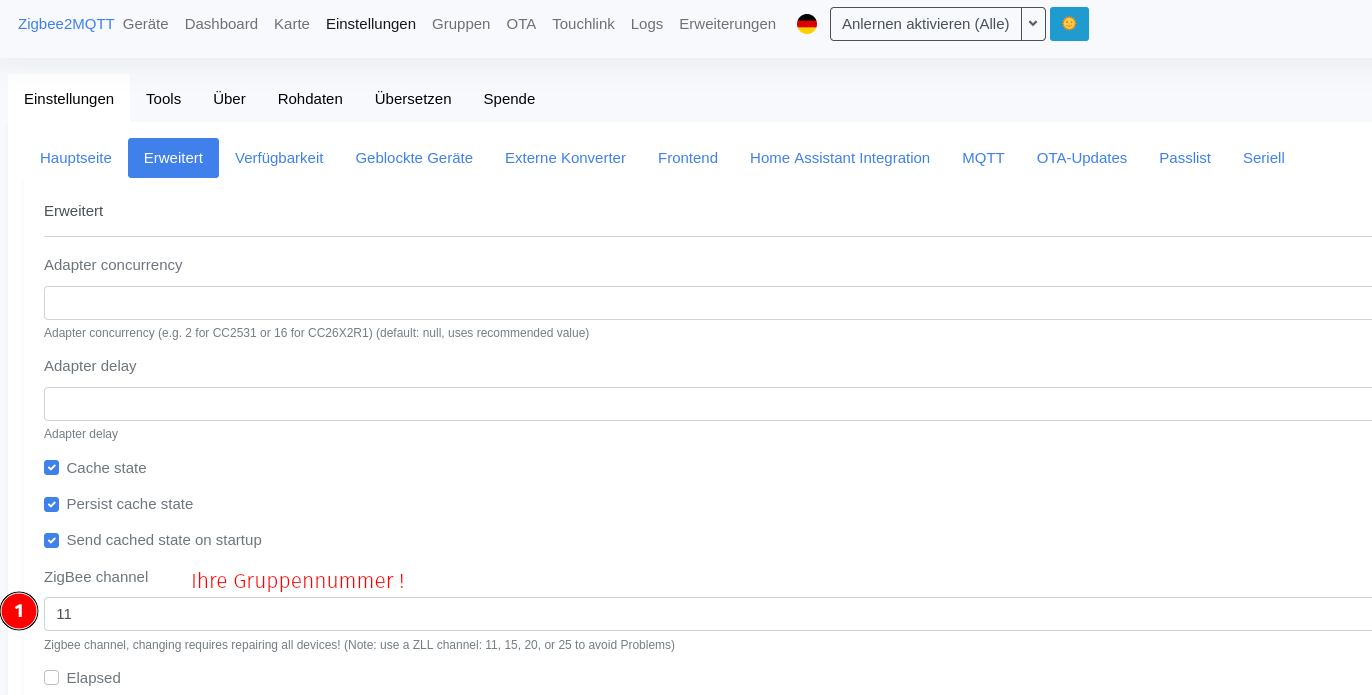
\includegraphics[width=1\textwidth]{media/Z2M-Channel.png}
    \caption{Zigbee Kanal Einstellung}
\end{figure}

Per Default verwendet Zigbee2Mqtt einen zufällig gewählten Netzwerkschlüssel. In dem Versuch wird der Schlüssel aber vorgegeben, um die Pakete
entschlüsseln zu können. Bitte setzen sie folgenden Schlüssel:

\begin{lstlisting}
    0x 00 00 ... 00 <Gruppe>
\end{lstlisting}

Die Einstellung finden sie unter der Kanal Einstellung als \grqq Network key(string)\grqq{}.

Achten sie darauf, im Anschluss die Einstellung am Ende der Seite zu bestätigen. Dafür klicken sie auf den 
\grqq Submit \grqq{} Button am Ende der Seite

\subsubsection{Wireshark Einrichtung}
Mit folgendem Befehl können sie ein Wireshak Capture auf entsprechenden Kanal starten:
Starten sie ein Konsolenfester und testen sie, ob der Befehl erfolgreich ausgeführt wird. Wireshark sollte starten, und Pakete sollten ersichtlich sein. Für \grqq 
<Kanal> \grqq{} setzen sie den von Ihnen gewählten Kanal ein.
\begin{lstlisting}
    > zbwireshark -c <Kanal>
\end{lstlisting}

Beenden sie den automatisch gestarteten Capture Vorgang. Gehen sie in das Menü: Bearbeiten > Einstellungen > Protokolle > ZigBee > Edit (Pre-configured Keys) und tragen
hier den \grqq TC-Link Key\grqq{} und den \grqq Network Key\grqq{} ein. Als \grqq Network Key\grqq{} verwenden sie den in Zigbee2Mqtt gesetzen Key. Der \grqq TC-Link Key\grqq{} ist ein
Standard-Key, der verwendet werden muss.
\begin{lstlisting}
    0x 5A 69 67 42 65 65 41 6C 6C 69 61 6E 63 65 30 39 (ZigBeeAlliance09)
\end{lstlisting}

Manche Hersteller verwenden proprietäre Schlüssel. Die Geräte sind dann nicht mit Koordinatoren anderer Hersteller Kompatibel.

\begin{Hinweis}
    Alle Aufgaben sollen mit Wireshark mitgeschnitten werden. Lesen sie die Aufgabenstellung erst durch und machen sie sich den Ablauf klar. Versuchen sie das 
    Zeitfenster des Wireshark Mitschnits so kurz wie möglich zu halten, und in dieser Zeit nur die in der Aufgabenstellung beschrieben Aktionen durchzuführen.
    Anderenfalls wird Ihr Mitschnitt sehr unübersichtlich.
\end{Hinweis}

\subsection{Aufgabe 2 - Joining einer Phillips Hue Lampe}

\subsubsection{Durchführung}
Schalten sie eine der beiden Zigbee Lampen ein. Die Lampe sollte leuchten. Dies ist das Standard verhalten, wenn die Lampen in keinem ZigBee Netz integriert sind.
Starten sie nun ein Wireshark Capture und erlauben in Zigbee2Mqtt das Anlernen von Geräten. Sobald Zigbee2Mqtt ein erfolgreiches Interview gemeldet hat, beenden sie
den Capture Vorgang. Die Lampe signalisiert durch ein kurzes blinken ebenfalls einen erfolgreiches Interview.

\begin{figure}[H]
    \centering
    
\includegraphics[width=1\textwidth]{media/Z2M-Anlernen.png}
    \caption{Zigbee Anlernen aktivieren}
\end{figure}

\begin{Hinweis}
    Speichern sie den Wireshark Capture ab als \textbf{\grqq <Gruppe> - ZigbeeLab - Aufgabe 2.1\grqq{}}
\end{Hinweis}

Navigieren sie nun zur Übersichtsseite der Lampe. Diese sollte ähnlich wie folgende Seite aussehen:

\begin{figure}[H]
    \centering
    \includegraphics[width=1\textwidth]{media/Z2M-Übersichtsseite.png}
    \caption{Zigbee Device Übersicht}
\end{figure}

Vergeben sie in der Übersichsseite der Lampe einen Nutzerfreundlichen namen. Die geschieht über den blauen Button im unteren Teil der Übersicht.
Dimmen und schalten sie die Lampe über die Weboberfläche. Die ist unter dem Reiter \grqq Details\grqq{} möglich. Starten sie einen weiteren Capture Vorgang, in dem sie einen Schaltvorgang mitschneiden.

\begin{Hinweis}
    Speichern sie den Wireshark Capture ab als \textbf{\grqq <Gruppe> - ZigbeeLab - Aufgabe 2.2\grqq{}}
\end{Hinweis}

\subsubsection{Fragen}

\subsubsection{Hinweise}
Sollte die Lampe sich nicht Verbinden, kann es notwendig sein die Lampe zurückzusetzen. In den FAQs finden sie zwei Methoden dazu.

\subsection{Aufgabe 3 - Joining einer Fernbedienung über die Lampe}

\subsection{Durchführung}
Für diese Aufgabe sollte nur die eine Lampe mit dem Koordinator verbunden sein. Die Fernbedienung wird nun über die Lampe dem Netzwerk hinzugefügt. Aus diesem Grund wird es nur der Lampe
erlaubt, ein neues Gerät aufzunehmen. Drücken sie den Setup Button auf der Fernbedienung, bis die LED dauerhaft grün leuchtet. Ein erfolgreiches anlernen wird auch hier in der Weboberfläche
und durch ein blinken der grünen LED signalisiert. Schneiden sie diesen Vorgang wieder mit Wireshark mit und speichern den Capture unter \grqq <Gruppe> - ZigbeeLab - Aufgabe3\grqq{}.

\begin{figure}[H]
    \centering
    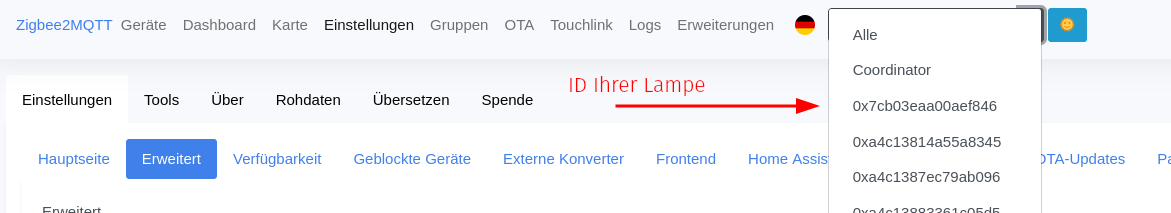
\includegraphics[width=1\textwidth]{media/Z2M-Anlernen-Lampe.png}
    \caption{Zigbee Anlernen aktivieren - nur Lampe}
\end{figure}

\begin{Aufgabe}
    Speichern sie den Wireshark Capture ab als \textbf{\grqq <Gruppe> - ZigbeeLab - Aufgabe 3\grqq{}}
\end{Aufgabe}

\subsubsection{Fragen}

\subsubsection{Hinweise}

\subsection{Aufgabe 4 - Binding der Fernbedienung}

\subsection{Durchführung}

Navigieren sie in der Weboberfläche zu der Übersicht Ihrer Lampe. Dort finden sie einen Reiter \grqq binden\grqq{}. Hier binden sie den Endpunkt X Ihrer Lampe mit dem Endpunkt X Ihrer Fernbedienung. 
Schalten sie nun die Lampe mit der Fernbedienung ein und aus. 

\begin{Hinweis}
    Speichern sie den Wireshark Capture ab als \textbf{\grqq <Gruppe> - ZigbeeLab - Aufgabe 4\grqq{}}
\end{Hinweis}

\subsection{Aufgabe 5 - Gruppenbildung}

\begin{Hinweis}
    Speichern sie den Wireshark Capture ab als \textbf{\grqq <Gruppe> - ZigbeeLab - Aufgabe 5\grqq{}}
\end{Hinweis}




